\documentclass[../TM3-UltraDoc.tex]{subfiles}
\begin{document}
	\section*{8) Hypergraphs}
	\addcontentsline{toc}{section}{8) Hypergraphs}
	% Your content here
	\textbf{Гиперграф (Hypergraph)} - граф, в котором ребра могут соединять любое количество вершин\\
	\\
	Также существуют ориентированные гиперграфы, в таком случае ребро выражается в виде подмножеств входных и выходных вершин\\
	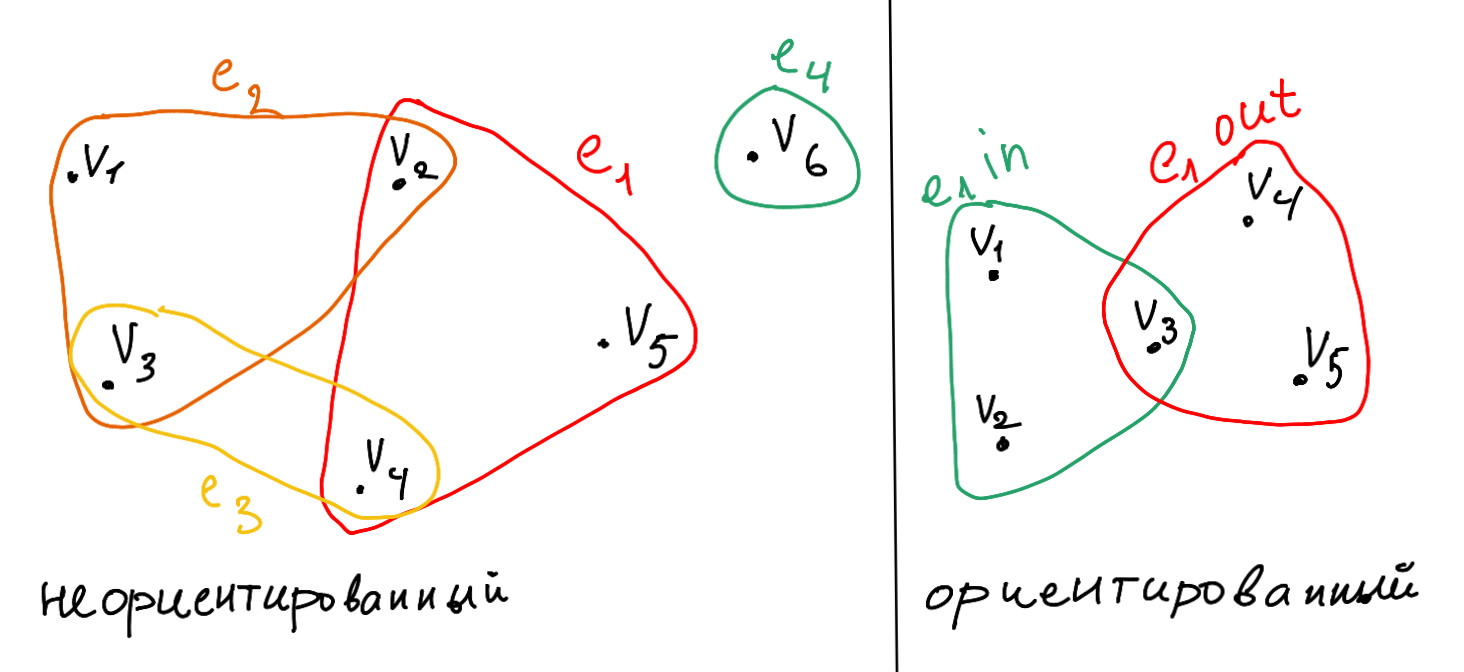
\includegraphics[width = 0.8\textwidth]{8.1}\\
	\begin{itemize}
		\item Неориентированный:\\
		\(
		V = \{v_1, v_2, v_3, v_4, v_5, v_6\}\\
		E = \{e_1, e_2, e_3, e_4\} = \{\{v_2, v_4, v_5\}, \{v_1, v_2, v_3\}, \{v_3, v_4\}, \{v_6\}\}
		\)
		\item Ориентированный:\\
		\(
		V = \{v_1, v_2, v_3, v_4, v_5\}\\
		E = \{e_1\} = \{\langle e^{\text{in}}_1, e^{\text{out}}_1 \rangle\} = \{\langle \{v_1, v_2, v_3\}, \{v_3, v_4, v_5\} \rangle\}
		\)
		
	\end{itemize}
	\end{document}